

%\subsubsection*{A storm-surge example}

\noindent{\bf Framework/Advancing Knowledge -- AIM 1:}
We illustrate our approach to Aim 1 with a concrete example. Consider the problem of predicting the maximum 
storm surge water level at a location (or locations) along a coast threatened by a cyclone. If we denote the geographical area of interest by $\Omega$ 
(the region threatened by the cyclone) and consider 
spatial points $(x,y) \in \Omega$. We restrict our interest to times $t$ in an interval of time $T = [t_0, t_1]$ (the duration of the storm). 
A mathematical model for storm surge is provided 
by the shallow water wave equations~\parencite{tan1992shallow}
\begin{subequations}
 \label{eqn:storm} 
\begin{align}
\frac{\partial h}{\partial t} +
\frac{\partial }{\partial x} \left(uh\right) + \frac{\partial }{\partial y} \left(vh\right) -R & =  0 ,\\
\frac{\partial uh}{\partial t} +
\frac{\partial }{\partial x} \left(u^2h +  \frac12 gh^2 \right) 
+ \frac{\partial }{\partial y} \left(vuh\right) + gh \frac{\partial b}{\partial x} 
- \frac{h}{\rho} \frac{\partial P}{\partial  x} - S_{fx} - S_{wx}  &= 0 ,   \\
\frac{\partial vh}{\partial t} +
\frac{\partial }{\partial x} \left(uvh  \right) 
+ \frac{\partial }{\partial y} \left(v^2h + \frac12 g h^2 \right) + gh \frac{\partial b}{\partial y} 
- \frac{h}{\rho} \frac{\partial P}{\partial  y} - S_{fy} -  S_{wy}& = 0,  
\end{align}
\end{subequations}
%\begin{subequations}
% \label{eqn:storm} 
%\begin{align}
%h_t + \mathbf{\nabla} \cdot (h  \mathbf{u} ) - R &= 0 \\
%( \mathbf{u}h)_t + \mathbf{\nabla} \cdot \left(h \mathbf{u} \otimes  \mathbf{u}  \right)  + gh \mathbf{\nabla} (h+b) - \frac{h}{\rho}  \mathbf{\nabla} P - \mathbf{S}_f - \mathbf{S}_w &=0
%\end{align}
%\end{subequations}
Here $h(x,y,t)$ is the depth of water and $u(x,y,t)$ and $v(x,y,t)$ are the $x$ and $y$ horizontal components of water velocity. 
The functions $h$, $u$ and $v$ are defined on the space/time domain  $ \mathcal{D} = \Omega \times T$. 
The equations include the graviational constant $g$ and the density of water $\rho$. Other terms constitute input data to the model: the bathymetry  (elevation of the ocean bed)  $b(x,y)$; the rate of rainfall on the region over time $R$; the atmospheric pressure $P$; %(which generates a surge due to spatial differences in atmospheric pressure associated with a large cyclone).
$S_{fx}$ and $S_{fy}$ the $x$ and $y$ components of the frictional force generated by the flow over the ocean bed 
%(flow over sand is different than flow through mangroves) 
 and $S_{wx}$ and $S_{wy}$ the $x$ and $y$ components of the surface stress force generated by the wind.


Our previous work~\parencite{anugamanual,nielsen2005hydrodynamic} has shown that these
equations, and their approximation using the  AnuGA package, provide a reliable
model of general flows associated with inundation due storm-surge as well as riverine flooding and tsunamis.
As is evident, there are many opportunities for uncertainty in the input data defining this model. 
If we denote by $\mathcal{P}$ the space representing the possible variation in both the {\bf input parameters} ($R$, $b$, $P$, $S_f$, $S_w$) and the {\bf design parameters} (emergency response actions such as raising or lowering flood barriers and releasing or diverting flow from upstream rivers or flood basins) then the aim of uncertainty quantification is to obtain useful relationships between the parameter vector $\mathbf{p}$
($\mathbf{p} \in \mathcal{P}$) and output quantities such as the maximum storm surge height as a function of location. 
A completely general parameter space $\mathcal{P}$ may lead to an intractable problem and it is sensible to look for a lower dimensional manifold $\mathcal{C} \subset \mathcal{P}$.
This can be done algorithmically or by using a specific reduced model, however, even such lower-dimensional approaches still necessitate numerous simulations of our model problem to quantify the uncertainty in our quantity of interest. {In addressing Aim 1}, we will study the shallow water wave equations in realistic flood inundation contexts in order to understand the relationship between their inputs and uncertainty and we will take advantage of new
developments combining sparse
grids~\parencite{BungartzGriebel2004}, reduced basis
methods~\parencite{LiebermanEtal2010,Peherstorfer2013,ChenSchwab2015,PeherstorferWillcox2015}
and uncertainty quantification.
 By using sparse
grids and reduced basis models we will be able to compute
\emph{surrogates of the full problem} which have significantly fewer
unknowns and are thus cheaper to compute whilst maintaining a high
order of accuracy. 
A sparse grid surrogate of
the model  can also be computed in an offline phase,
so that in an online phase model solutions can be efficiently
estimated using the surrogate model and for many problems sparse grids
can also be used over $\mathcal{D}$ when computing solutions to the full
model to speed up the construction of a reduced basis.\\

%We will compute
%sparse grid solutions via the `combination
%technique'~\parencite{Griebel1990}. 

 \iffalse
 
 Figure~\ref{fig:sparse_grids}
depicts the combination technique, the equivalent sparse grid and the
corresponding full grid.
 
 \begin{figure}
  \centering
  % Brendan: combination grid, sparse grid, fullgrid figure

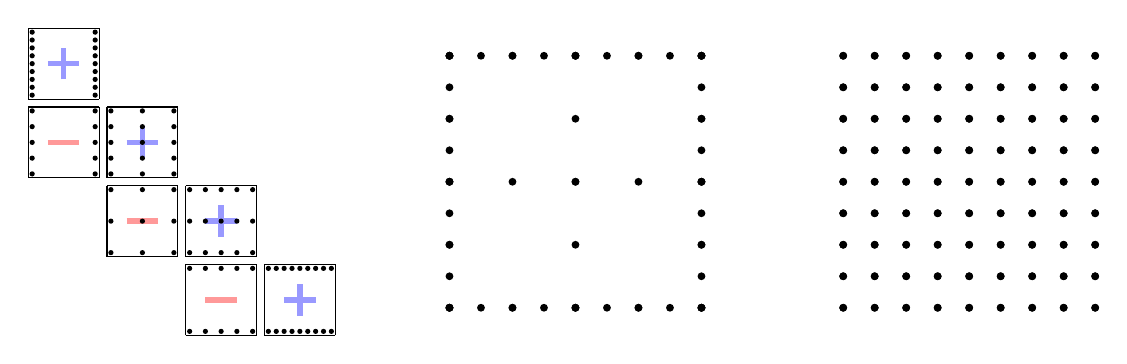
\begin{tikzpicture}%[scale=0.8]
%\scriptsize
%%% Draw squares around component grids
\foreach \i in {1,...,4}
{
	\pgfmathtruncatemacro{\x}{(\i - 1)};
	\draw[] (0.05+1.0*\x, 3.05-1.0*\x) -- (0.05+1.0*\x+0.9, 3.05-1.0*\x) {};
	\draw[] (0.05+1.0*\x, 3.05-1.0*\x) -- (0.05+1.0*\x, 3.05-1.0*\x+0.9) {};
	\draw[] (0.05+1.0*\x+0.9, 3.05-1.0*\x) -- (0.05+1.0*\x+0.9, 3.05-1.0*\x+0.9) {};
	\draw[] (0.05+1.0*\x, 3.05-1.0*\x+0.9) -- (0.05+1.0*\x+0.9, 3.05-1.0*\x+0.9) {};
	%%% optional plotting of coefficients
	\draw[blue!40,line width=0.7mm] (0.5+1.0*\x-0.2, 3.0+0.5-1.0*\x) -- (0.5+1.0*\x+0.2, 3.0+0.5-1.0*\x);
	\draw[blue!40,line width=0.7mm] (0.5+1.0*\x, 3.0+0.5-1.0*\x-0.2) -- (0.5+1.0*\x, 3.0+0.5-1.0*\x+0.2);
}
\foreach \i in {1,...,3}
{
	\pgfmathtruncatemacro{\x}{(\i - 1)};
	\draw[] (0.05+1.0*\x, 2.05-1.0*\x) -- (0.05+1.0*\x+0.9, 2.05-1.0*\x) {};
	\draw[] (0.05+1.0*\x, 2.05-1.0*\x) -- (0.05+1.0*\x, 2.05-1.0*\x+0.9) {};
	\draw[] (0.05+1.0*\x+0.9, 2.05-1.0*\x) -- (0.05+1.0*\x+0.9, 2.05-1.0*\x+0.9) {};
	\draw[] (0.05+1.0*\x, 2.05-1.0*\x+0.9) -- (0.05+1.0*\x+0.9, 2.05-1.0*\x+0.9) {};
	%%% optional plotting of coefficients
	\draw[red!40,line width=0.7mm] (0.5+1.0*\x-0.2, 2.0+0.5-1.0*\x) -- (0.5+1.0*\x+0.2, 2.0+0.5-1.0*\x);
}
%%% Combination grids
\foreach \i in {1,...,18} %2*9
{
	\pgfmathtruncatemacro{\y}{(\i - 1) / 2};
	\pgfmathtruncatemacro{\x}{\i - 1 - 2 * \y};
	\node[fill,circle,scale=0.2] at (0.1+0.8*\x,3.1+0.1*\y) {};
	\node[fill,circle,scale=0.2] at (3.1+0.1*\y,0.1+0.8*\x) {};
}
\foreach \i in {1,...,15} %3*5
{
	\pgfmathtruncatemacro{\y}{(\i-1)/3};
	\pgfmathtruncatemacro{\x}{\i-1-3*\y};
	\node[fill,circle,scale=0.2] at (1.1+0.4*\x,2.1+0.2*\y) {};
	\node[fill,circle,scale=0.2] at (2.1+0.2*\y,1.1+0.4*\x) {};
}
\foreach \i in {1,...,10} %2*5
{
	\pgfmathtruncatemacro{\y}{(\i-1)/2};
	\pgfmathtruncatemacro{\x}{\i-1-2*\y};
	\node[fill,circle,scale=0.2] at (0.1+0.8*\x,2.1+0.2*\y) {};
	\node[fill,circle,scale=0.2] at (2.1+0.2*\y,0.1+0.8*\x) {};
}
\foreach \i in {1,...,9} %3*3
{
	\pgfmathtruncatemacro{\y}{(\i - 1) / 3};
	\pgfmathtruncatemacro{\x}{\i - 1 - 3 * \y};
	\node[fill,circle,scale=0.2] at (1.1+0.4*\x,1.1+0.4*\y) {};
}
%%% Sparse grid
\foreach \i in {1,...,18} %2*9
{
	\pgfmathtruncatemacro{\y}{(\i - 1) / 2};
	\pgfmathtruncatemacro{\x}{\i - 1 - 2 * \y};
	\node[fill,circle,scale=0.3] at (5.4+3.2*\x,0.4+0.4*\y) {};
	\node[fill,circle,scale=0.3] at (5.4+0.4*\y,0.4+3.2*\x) {};
}
\foreach \i in {1,...,15} %3*5
{
	\pgfmathtruncatemacro{\y}{(\i-1)/3};
	\pgfmathtruncatemacro{\x}{\i-1-3*\y};
	\node[fill,circle,scale=0.3] at (5.4+1.6*\x,0.4+0.8*\y) {};
	\node[fill,circle,scale=0.3] at (5.4+0.8*\y,0.4+1.6*\x) {};
}
%%% Full grid
\foreach \i in {1,...,81} %9*9
{
	\pgfmathtruncatemacro{\y}{(\i - 1) / 9};
	\pgfmathtruncatemacro{\x}{\i - 1 - 9 * \y};
	\node[fill,circle,scale=0.3] at (10.4+0.4*\x,0.4+0.4*\y) {};
	\node[fill,circle,scale=0.3] at (10.4+0.4*\y,0.4+0.4*\x) {};
}
\end{tikzpicture}  
  \caption{Combination grids on the left (with coefficients, marked with
    a blue plus for $+1$ and red minus for $-1$), sparse grid in the
    middle, full grid on the right. Note the marked reduction in the number of 
    grid points for the sparse grid relative to the full grid. 
   This is even more pronounced in higher dimensions.}
  \label{fig:sparse_grids}
\end{figure}
\fi

 \iffalse
The model solution 
$$
U_{\mathbf{p}} (\mathbf{x})  = (  h(x,y,t) , u(x,y,t) ,  v(x,y,t) )
$$
represents the water depth and velocity fields obtained by solving the model problem for a choice of parameter $\mathbf{p}$ at a particular location and time $\mathbf{x} = (x,y,t)$.
Equation~\eqref{eqn:storm} can be characterised as $M_{\mathbf{p}}(U_{\mathbf{P}}) = 0$.

In this case, the quantity of interest $Q(U_{\mathbf{p}})$ will be the maximum storm surge height at a particular location $(x_0, y_0) \in \Omega$,
$$ 
Q(U_{\mathbf{p}})  = \max_{t_0 \leq t \leq t_1} \left( h(x_0,y_0,t) + b(x_0,y_0) \right).
$$
The aim of  uncertainty quantification is to obtain useful relationships between the variations in pressure, wind and rainfall (changes of $\mathbf{p} \in \mathcal{P}$) and $Q(U_{\mathbf{p}})$, including identifying which components of the inputs  have the greatest influence on the result. 



A completely general parameter space $\mathcal{P}$ may lead to an intractable problem. It is sensible to look for a lower dimensional manifold $\mathcal{C} \subset \mathcal{P}$. This can be done algorithmically. Or in this case $\mathcal{C}$ might represent a model of the pressure, wind and rainfall associated with a cyclone of specific intensity and location. This would still involve uncertainty, and so would entail numerous solutions of our model problem to quantify the uncertainty in our quantity of interest. Finally, as we investigate our model, it might be advantageous to change the assumptions of our cyclone model, or incorporate updated forecasts or indeed play with adding different types of uncertainty to the various input data streams. This is where live programming and real time interaction with our model becomes paramount. 
\fi